\documentclass{fduthesis}

\usepackage{bm}
\usepackage{graphicx}
\usepackage{float}
\usepackage{fontspec}
\usepackage{booktabs}
\graphicspath{{figures/}{}}
\usepackage{amsfonts}
\usepackage{amsmath}

\renewcommand\thesection{\arabic{section}} 
\renewcommand {\thetable} {\thesection{}.\arabic{table}}
\renewcommand {\thefigure} {\thesection{}.\arabic{figure}}

\fdusetup{
  style = {
    font-size = 5,
    fullwidth-stop = catcode,
    auto-make-cover = false}
}

\title{信息论 project\\JPEG2000}
\author{高云帆\\张奕朗 16307130242\\陈幸豪 16307130006}
\date{\today}

\begin{document}
\maketitle

\section{综述}

%\subsection{整体流程}

%\subsection{分工}
高云帆:\par
张奕朗:\par
陈幸豪:色彩空间变换,量化,搭整个程序的框架,设计协调整个流程的数据结构。

\section{图像分块与电平平移归一化}

在图像变换之前,首先需要对图像进行预处理。预处理主要分为分块、电平平移归一化和颜色变换三个过程(\textbf{图\ref{fig1}})。在调用\textit{cv2.imread}读取图像数据时,利用正则表达式获取图像的颜色位数信息,方便之后的处理。\textit{代码见函数init\_image。}

\begin{figure}[H]
	\centering
	
\includegraphics[scale=0.4]{fig1}
	\caption{图像预处理.}
	\label{fig1}
\end{figure}

\subsection{图像分块}
与JPEG标准相同,JPEG2000标准也需要将图像分块,不过是为了降低计算量和对内存的需求,以方便压缩(当然也可以选择不分块)。但与JPEG标准不同的是,JPEG2000标准并不需要将图像强制分成$8\times 8$的小块,而是可以将图像分割成若干任意大小的互不重叠的矩形块(tile),常分为$2 ^6\sim 2^{12}$(即$64\sim 1024$像素宽)的正方形tile。受图像形状的影响,边缘部分的tile的大小和形状可能与其它的tile不同。Tile的大小会影响重构图像的质量。一般情况下,大的tile重构出的图像质量要好一些,因为小波变换的范围大,减轻了边缘效应。\textit{代码见class Tile和class JPEG2000中的函数image\_tiling。} \par

\subsection{电平平移归一化}
电平平移归一化分为两步:\par
第一步是直流电平平移(DC level shifting),通过将数据减去均值使之关于0对称分布,以去掉频谱中的直流分量。
\[
\begin{aligned}
I_1(x,y)=I(x,y)-2^{B-1}\\
-2^{B-1}\le I_1(x,y)\le 2^{B-1}-1
\end{aligned}
\]
其中B是之前读取到的颜色位数信息。\par
第二步是电平归一化(normaliztion)。对于无损压缩中的5/3小波变换,由于采用的是整数小波变换,所以不需要进行归一化;而对于有损压缩中的9/7小波变换,由于采用的是实数小波变换,故需要对每个tile进行如下运算以归一化:\par
\[
\begin{aligned}
I_2(x,y)=\frac{I_1(x,y)}{2^{B}}\\
-\frac{1}{2}\le I_2(x,y)<\frac{1}{2}
\end{aligned}
\]
但是事实上,电平平移归一化对DWT来说不是必须的(而且电平平移归一化后还不便于进行色彩空间变换),因为它只会影响小波系数的动态范围而不会影响结果。\textit{代码见函数dc\_level\_shift。}

\subsection{反变换}
在解码、小波反变换和色彩空间反变换之后,需要进行电平反平移,(如果是有损压缩,还需要进行反归一化),最后拼接得到恢复的图像。这些都是上述操作的反过程,这里不再赘述。\textit{代码见函数idc\_level\_shift和image\_splicing。}





\section{颜色空间变换}

通常所谓的颜色由红绿蓝(RGB)组成,即RGB形成了颜色空间的一组基。其他常用颜色空间有CMY,HSV,YCbCr等。JPEG2000标准中,可以选择将RGB颜色变换到其他空间。需要注意的是,图像可能有超过3个颜色分量,而JPEG2000的颜色变换只运用于前3个颜色分量。此外,变换过程在理论上不区分输入的颜色空间,即输入颜色不一定须为RGB数据。颜色空间变换的目的是利用三个图像分量组合之间的冗余。例如人眼对YCbCr空间的Y分量更敏感,而对Cb、Cr分量相对不敏感。此时可对Y分量做无损压缩,而对CbCr做有损压缩。此时图片的体积可被减小,而观感相比无损压缩没有明显损失。\par

JPEG2000定义了不可逆彩色变换(ICT)和可逆彩色变换(RCT)。ICT计算过程中使用的小数难以被二进制精确表示,即必然存在计算误差。因此无损压缩必须使用RCT。代码中颜色空间变换的函数名为\textit{component\_transformation},可按压缩方式选择ICT或RCT。下面分别介绍两种变换。

\subsection{ICT}
ICT可视为一个线性变换。它将归一化到$\left[-\frac{1}{2}, \frac{1}{2}\right]$的RGB彩色变换到YCbCr空间。首先定义以下加权因子
\begin{equation}
\begin{aligned}
\alpha_R=0.299, \alpha_G=0.587,\alpha_B=0.114
\end{aligned}
\end{equation}
以及变换关系
\begin{equation}
\begin{aligned}
x_{Y}[n]=\alpha_{R}x_{R}[n]+\alpha_{G}x_{G}[n]+\alpha_{B}x_{B}[n]\\
x_{Cb}[n]=\frac{0.5}{1-\alpha_B}(x_{B}[n]-x_{Y}[n])\\
x_{Cr}[n]=\frac{0.5}{1-\alpha_B}(x_{R}[n]-x_{Y}[n])
\end{aligned}
\end{equation}
这一关系可用矩阵表示如下
\begin{equation}
\begin{aligned}
\left(
\begin{array}{c}
x_{Y}[n]\\
x_{Cb}[n]\\
x_{Cr}[n]
\end{array}
\right)
=
\left(
\begin{array}{ccc}
0.299 & 0.587 & 0.114\\
-0.168736 & -0.331264 & 0.5\\
0.5 & -0.418688 & -0.081312
\end{array}
\right)
\left(
\begin{array}{c}
x_{R}[n]\\
x_{G}[n]\\
x_{B}[n]
\end{array}
\right)
\end{aligned}
\end{equation}

需要注意,以上矩阵中使用的小数都是近似值。实际计算中,所有数值必须精确处理。\par
在有损压缩中,若输入的RGB值域已被归一化到$\left[-\frac{1}{2}, \frac{1}{2}\right]$,则不难证明,输出的YCbCr值域也在$\left[-\frac{1}{2}, \frac{1}{2}\right]$。其中$x_{Y}$是RGB分量的加权平均,被认为是图像强度(或亮度)的量度。该权重了反映可见光谱中绿色段信息对于视觉感知的重要性。\par

解压缩过程中,对应的ICT反变换如下

\begin{equation}
\begin{aligned}
\left(
\begin{array}{c}
x_{R}[n]\\
x_{G}[n]\\
x_{B}[n]
\end{array}
\right)
=
\left(
\begin{array}{ccc}
1 & 0 & 1.402\\
1 & -0.344136 & -0.714136\\
1 & 1.772 & 0
\end{array}
\right)
\left(
\begin{array}{c}
x_{Y}[n]\\
x_{Cb}[n]\\
x_{Cr}[n]
\end{array}
\right)
\end{aligned}
\end{equation}
其中仅第1行和第3行的小数为精确值。\par

ICT反变换不具有正向变换的范围保持特性。此外,由于输入的$x_{Y}[n]$、$x_{Cb}[n]$和$x_{Cr}[n]$通常已被量化所损坏,所以由ICT反变换重建的RGB值不一定落在$\left[-\frac{1}{2}, \frac{1}{2}\right]$。
解压缩程序可对超出范围的RGB样本值进行处理,但JPEG2000标准并未指定处理方法。\par

\subsection{RCT}
RCT将值域为$\left[-2^B, 2^B-1\right]$的RGB彩色变换到Y'DbDr空间。RCT由以下非线性关系定义
\begin{equation}
\begin{aligned}
x_{Y}'[n]&=\left \lfloor \frac{x_{R}[n]+2x_{G}[n]+x_{B}[n]}{4} \right \rfloor\\
x_{Db}[n]&=x_{B}[n]-x_{G}[n]\\
x_{Dr}[n]&=x_{R}[n]-x_{G}[n]
\end{aligned}
\end{equation}

其中$\left \lfloor \textit{x} \right \rfloor$表示小于等于\textit{x}的最大整数。\par
可以证明RCT能被精确地反变换。由于
\begin{equation}
\begin{aligned}
\left \lfloor \frac{x_{Db}[n]+x_{Dr}[n]}{4} \right \rfloor
&=\left \lfloor \frac{x_{R}[n]+2x_{G}[n]+x_{B}[n]}{4}-x_{G}[n] \right \rfloor\\
&=x_{Y}'[n]-x_{G}[n]
\end{aligned}
\end{equation}
因此我们可以先重建$x_{G}[n]$,再借此重建$x_{R}[n]$和$x_{B}[n]$。定义RCT反变换为
\begin{equation}
\begin{aligned}
x_{G}[n]&=x_{Y}'[n]-\left \lfloor \frac{x_{Db}[n]+x_{Dr}[n]}{4} \right \rfloor\\
x_{B}[n]&=x_{Db}[n]+x_{G}[n]\\
x_{R}[n]&=x_{Dr}[n]+x_{G}[n]
\end{aligned}
\end{equation}

RCT也可以近似取一种变换关系如下
\begin{equation}
\begin{aligned}
\left(
\begin{array}{c}
x_{Y}'[n]\\
x_{Db}[n]\\
x_{Dr}[n]
\end{array}
\right)
=
\left(
\begin{array}{ccc}
0.25 & 0.5 & 0.25\\
0 & -1 & 1\\
1 & -1 & 0
\end{array}
\right)
\left(
\begin{array}{c}
x_{R}[n]\\
x_{G}[n]\\
x_{B}[n]
\end{array}
\right)
\end{aligned}
\end{equation}
其反变换可近似为
\begin{equation}
\begin{aligned}
\left(
\begin{array}{c}
x_{R}[n]\\
x_{G}[n]\\
x_{B}[n]
\end{array}
\right)
=
\left(
\begin{array}{ccc}
1 & -0.25 & -0.25\\
1 & -0.25 & 0.75\\
1 & 0.75 & -0.25
\end{array}
\right)
\left(
\begin{array}{c}
x_{Y}'[n]\\
x_{Db}[n]\\
x_{Dr}[n]
\end{array}
\right)
\end{aligned}
\end{equation}
这里的近似仅仅修改了变换关系,没有对任何数值进行舍入处理。所以近似变换依然是无损的。

\section{小波变换}
\subsection{小波变换原理简述}
对非平稳过程,傅里叶变换有其局限性。它只能获取一段信号总体上包含哪些频率的成分,但是对各成分出现的时刻并无所知。因此时域相差很大的两个信号,可能频谱图一样。而加窗截取信号的STFT(短时傅里叶变换)又存在窗长的问题:窗太窄,频率分辨率差;窗太宽,时间分辨率低。于是便产生了利用有限长的会衰减的小波基进行与源信号进行相关的WT(小波变换)和DWT(离散小波变换),需要用到的DWT的变换和逆变换公式如下:
\[
\begin{aligned}
WT[j,k]=\sum_n\langle f,\psi_{j,k}\rangle=\frac{1}{\sqrt{j}}\sum_{n}f[n]\psi[\frac{n-k}{j}]\\
f[n]=\sum_{j,k}\langle f,\psi_{j,k}\rangle\hat{\psi}_{j,k}=\frac{1}{A}\sum_{j,k}WT[j,k]\psi_{j,k}
\end{aligned}
\]

不同于傅里叶变换,变量只有频率$\omega$,小波变换有两个变量:尺度j和平移量 k。尺度j控制小波函数的伸缩,平移量k控制小波函数的平移。尺度j对应于频率(反比),平移量k对应于时间。

\begin{figure}[H]
	\centering
	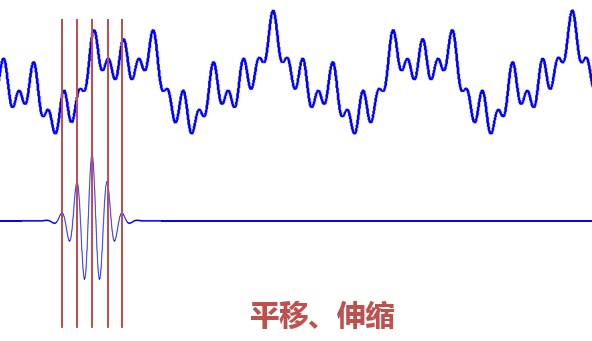
\includegraphics[scale=0.4]{fig2}
	\caption{小波基的尺度参数和平移参数.}
	\label{fig2}
\end{figure}

\subsection{小波变换的滤波器实现与提升算法}
\subsubsection{小波变换的滤波器等效}
小波变换可以用IIR滤波器进行等效(具体推导见《JPEG2000图像压缩基础、标准和实践》),并且可以通过提升算法进行实现。在有损压缩的情况下,JPEG2000标准的核心编码系统默认的不可逆小波变换是Daubechies 9/7 DWT的提升实现,而在无损情况下则采用Le Gall 5/3滤波器的提升实现的整数可逆小波变换。其中Daubechies 9/7是I.Daubechies与M.Antonini等人于1992年提出的一种双正交小波滤波器。Le Gall 5/3是D.Le Gall 与 A.Tabatabai于1988年基于样条5/3变换而提出的一种可逆双正交滤波器。两者的滤波器参数见\textbf{图\ref{fig3}、\ref{fig4}}。其中参数9/7和5/3分别指分解低/高通滤波器的IIR长度,合成滤波器相反(正交对称)。

\begin{figure}[H]
	\centering
	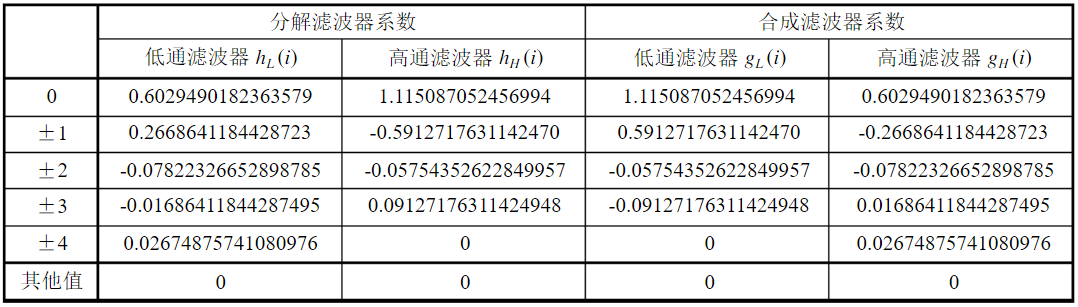
\includegraphics[scale=0.6]{fig3}
	\caption{Daubechies 9/7 滤波器系数表.}
	\label{fig3}
\end{figure}

\begin{figure}[H]
	\centering
	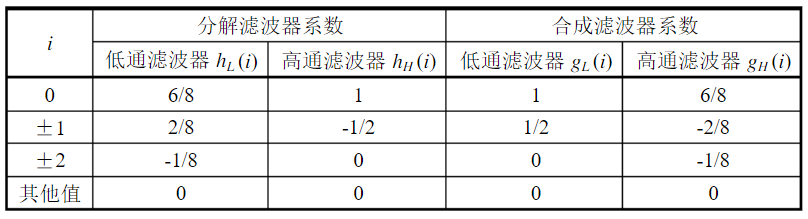
\includegraphics[scale=0.7]{fig4}
	\caption{Le Gall 5/3 滤波器系数表.}
	\label{fig4}
\end{figure}

\subsubsection{小波变换的提升算法}
\paragraph{Daubechies 9/7} 正变换包括4步提升和2步缩放:\par
4步提升:
\[
\begin{aligned}
y(2n+1)&=x(2n+1)-\alpha[x(2n)+x(2n+2)]\\
y(2n)&=x(2n)-\beta[y(2n-1)+y(2n+1)]\\
y(2n+1)&=y(2n+1)+\gamma[y(2n)+y(2n+2)]\\
y(2n)&=y(2n)+\delta[y(2n-1)+y(2n+1)]
\end{aligned}
\]\par
2步缩放:
\[
\begin{aligned}
y(2n+1)&=-Ky(2n+1)\\
y(2n)&=y(2n)/K
\end{aligned}
\]\par

逆变换包括2步缩放和4步提升:\par
2步缩放:
\[
\begin{aligned}
x(2n+1)&=-y(2n+1)/K\\
x(2n)&=Ky(2n)
\end{aligned}
\]\par
4步提升:
\[
\begin{aligned}
x(2n)&=x(2n)-\delta*[x(2n-1)+x(2n+1)]\\
x(2n+1)&=x(2n+1)-\gamma*[x(2n)+x(2n+2)]\\
x(2n)&=x(2n)+\beta*[y=x(2n-1)+x(2n+1)]\\
x(2n+1)&=x(2n+1)+\alpha*[x(2n)+x(2n+2)]
\end{aligned}
\]\par


其中 $\alpha,\beta,\gamma,\delta,K$ 为与滤波器系数有关的参数:$\alpha=1.586134342,\beta=0.052980118,\gamma=0.882911075,\delta=0.443506852,K=1.230174105$。

\paragraph{Le Gall 5/3} 正、逆变换均只需要一步提升与一步缩放。\par
正变换:
\[
\begin{aligned}
y(2n+1)&=x(2n+1)-[x(2n)+x(2n+2)]/2\\
y(2n)&=x(2n)+[y(2n-1)+y(2n+1)+2]/4
\end{aligned}
\]
逆变换:
\[
\begin{aligned}
x(2n)&=y(2n)-[y(2n-1)+y(2n+1)+2]/4\\
x(2n+1)&=y(2n+1)+[x(2n)+x(2n+2)]/2
\end{aligned}
\]

\subsection{二维多级小波变换}
对图像进行2D-DWT后可得到图像的2D-DWT系数,将系数按照左上、左下、右上、右下分别分为LL、LH、HL、HH四个分量(L表示低频,H表示高频)。由于图像的信息大多集中在低频区域,所以若分解所得的LL分量仍含有较多的图像信息时(动态范围大,不利于量化和编码),可将其进一步做2D-DWT分解,也就是多级小波分解,如\textbf{图\ref{fig5}}所示。JPEG2000中一般做$3\sim 4$级2D-DWT,经实践,选用3级2D-DWT就已经足够了。

\begin{figure}[H]
	\centering
	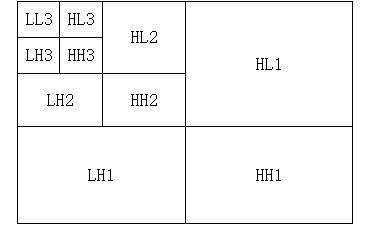
\includegraphics[scale=0.6]{fig5}
	\caption{二维小波变换的多级划分.}
	\label{fig5}
\end{figure}
开始时我用\textit{for}循环实现了提升算法,但是运行速度太慢,于是改为调用\textit{python}的PyWavelets包,建立自定义小波来实现2D-DWT。虽然Daubechies 9/7是以Daubechies命名的,但它和普通的DB族小波基都不同:普通的DB小波基是非对称非正交小波基,而Daubechies 9/7是双正交对称小波基,在查阅官方的小波库文档之后,重新按照双正交对称小波基的参数进行排列,最终实现了基于DB 9/7(有损情况)和LG 5/3滤波器(无损情况)的2D-DWT和2D-iDWT,且速度较原来\textit{for}循环的算法有了很大的提升。\textit{代码见函数dwt和idwt。}




\section{量化}

JPEG2000中的量化是将小波系数的大量可能的离散取值近似为较少个离散值的过程,即小波子带的样本通过量化过程映射到量化索引中。本文用$Q(x)$表示对$x$量化所得的值,而反量化表示为$\hat{x}=\overline{Q^{-1}}(Q(x))$。非细小的量化本身是不可逆的,所以JPEG2000的无损压缩中不包括量化。但在对小波系数进行编码时,不论有损或无损压缩,我们都必须为编码器提供待编码数值的一致解释,称为界定(ranging)。有损压缩中,量化本身就是一种界定过程。而无损压缩需要一段独立程序来完成界定。代码中的量化的核心函数名为\textit{quantization\_math},入口函数名逐次为\textit{quantization}和\textit{quantization\_helper}。\par
不同的量化策略对画质和码率的影响很大。限于个人水平和时间,加上小波系数的“概率分布”难以描述,且为了保险起见(复杂的量化策略会带来复杂的数据结构,而量化过程承上启下,数据结构不容出错)(事实上确实出错了一次,用递归方式修正回来了),我们只在程序中对有损压缩使用了最简单的标量均匀量化器,而无损压缩不经过量化或界定。均匀量化的性能并非最佳,但我们可以通过优化均匀量化方式来提升相同比特率下的显示效果。

\subsection{标量量化}
标量量化(SQ)是最简单的处理方式。它将实轴的一个子集中的每一个元素映射为该子集中的一个特定值。考虑将实轴划分为M个不相交的区间
\begin{equation}
\begin{aligned}
I_{q}=[t_{q},t_{q+1}),q=0,1,...,M-1
\end{aligned}
\end{equation}
其中
\begin{equation}
\begin{aligned}
-\infty=t_{0}<t_{1}<...<t_{M}=+\infty
\end{aligned}
\end{equation}
在每个区间内,选择点$x_{q}$作为$I_{q}$的输出值,则可将标量量化器理解为从$\mathbb{R}$到${0,1,,...,M-1}$的映射。对一个给定的$x$,$Q(x)$是包含x的区间$I_{q}$的索引。均匀量化的反量化器由
\begin{equation}
\begin{aligned}
\overline{Q^{-1}}(q)=x_{q}
\end{aligned}
\end{equation}
给出。

\subsection{标量量化器的优化:Lloyd-Max标量量化}
若要求$Q(x)$所有可能取值的个数$M$是固定不变的,则我们可以根据某些条件来优化量化过程。满足这些条件的量化器称为Lloyd-Max量化器。我们假定一个平稳过程具有边缘概率密度函数$f_{X}$,并采用均方误差(MSE)来度量失真。则有
\begin{equation}
\begin{aligned}
\text{MSE}&=E\left[(X-\hat{X})^{2}\right]\\
&=\sum\limits_{q = 0}^{M - 1} {E\left[(X-\hat{X})^{2}|X \in I_{q}\right]P(X \in I_{q})}\\
&=\sum\limits_{q = 0}^{M - 1} {\int_{{t_q}}^{{t_{q+1}}} {{{(x - \hat{x}_q)}^2}{f_X}(x)dx} }
\end{aligned}
\end{equation}
若要求$\frac{\partial (\text{MSE})}{\partial {t_q}}=0$,即${({t_q} - \hat{x}_{q-1})^2}{f_x}({t_q}) - {({t_q} - \hat{x}_q)^2}{f_x}({t_q}) = 0$,可解得
\begin{equation}
t_q=\frac{\hat{x}_{q-1}+\hat{x}_{q}}{2}, q=1,2,...,M-1\label{eqn:tq}
\end{equation}
类似地,由$\frac{\partial (\text{MSE})}{\partial {\hat{x}_q}}=0$解得
\begin{equation}
\hat{x}_{q}=\frac{\int_{{t_q}}^{{t_{q+1}}} {x{f_X}(x)dx}}{\int_{{t_q}}^{{t_{q+1}}} {{f_X}(x)dx}}, q=1,2,...,M-1\label{eqn:xq}
\end{equation}
式(\ref{eqn:tq})和(\ref{eqn:xq})构成优化标量量化器的必要条件。(\ref{eqn:tq})表明量化器决策区域的端点应该在输出点的中间(不是“输出点在端点之间”!)。(\ref{eqn:xq})的分母是$X$位于$I_{q}$中的概率,由此可得
\begin{equation}
\hat{x}_q=E\left[X|X \in I_{q}\right]
\end{equation}
满足这一性质的码字称为“条件均值”或“质心”。\par
此外,由式(\ref{eqn:tq})和(\ref{eqn:xq})可得以下性质
\begin{equation}
E[X-\hat{X}]=0
\end{equation}
\begin{equation}
\sigma_{\hat{X}}^2= \sigma_{X}^2-E[(X-\hat{X})^2]
\end{equation}
\begin{equation}
E[(X-\hat{X})\hat{X}]=0
\end{equation}
\begin{equation}
E[(X-\hat{X})^2|X \in I_{j}]P(X \in I_{j})=E[(X-\hat{X})^2|X \in I_{q}]P(X \in I_{q}), \forall j,q
\end{equation}
这些性质分别说明:量化误差均值为0(不论是否有$E(X)=0$);量化使数据方差减小的量等于均方误差;量化误差与量化器输出无关(但不是与输入无关);所有区间对量化误差的贡献相等。\par
式(\ref{eqn:tq})和(\ref{eqn:xq})只是必要条件,因此不能保证最优化。但对于所有对数凹概率密度函数(即$\log f_{X}$是凹函数或凸函数),最优化是可以保证的[7]。幸运的是,均匀分布、拉普拉斯分布和正态分布都满足这一性质。另外,在均匀量化的基础上,我们可以对某些量化区间再进行均匀划分。这样就构造了一族嵌入均匀标量量化器。可以证明,这些量化器全部满足均匀分布的Lloyd-Max条件。

\subsection{恒域量化}
显然,步长为$\Delta$的均匀量化
\begin{equation}
I_{q}=\left[q\Delta-\frac{\Delta}{2},q\Delta+\frac{\Delta}{2}\right)
\end{equation}
一般不是最优量化,然而具有均匀区间,且质心码字为$\hat{x}_{q}=E[X|X \in I_{q}]$的量化器是非常接近最优量化的[8]。对于零均值概率密度函数,如果在均匀量化基础上加宽以0为中心的区间,常常可以使MSE性能获得改进,并减小量化输出值的熵$H(\hat{X})$。被加宽的零均值区间$I_{0}$有时被称为“储零箱(zero-bin)”。这种量化称为“恒域(deadzone)均匀标量量化”。其数学描述为
\begin{equation}
I_{q}=\left\{
\begin{aligned} %一定要有\begin{aligned}
&\left[-(1-\xi)\Delta, (1-\xi)\Delta\right), &q=0\\
&\left[(q-\xi)\Delta, (q+1-\xi)\Delta\right), &q>0\\
&\left[(q-1+\xi)\Delta, (q+\xi)\Delta\right), &q<0\\
\end{aligned}
\right.
\end{equation}
其中$\xi<1$决定$I_{0}$的宽度。这个量化器的具体实现为
\begin{equation}
q=Q(x)=\left\{
\begin{aligned} %一定要有\begin{aligned}
&\text{sgn}(x)\left\lfloor \frac{|x|}{\Delta}+\xi\right\rfloor, &\frac{|x|}{\Delta}+\xi>0\\
&0, &\text{其他}\\
\end{aligned}
\right.
\end{equation}

JPEG2000标准要求小波子带样本$b$可被恒域量化($b$可代表LL,LH,HL,HH),且中央量化间隔(即恒域)是其他量化间隔的2倍。此时有$\xi=0$,即
\begin{equation}
q_{b}[n]=\text{sgn}(y_{b}[n])\left\lfloor\frac{|y_{b}[n]|}{\Delta_{b}}\right\rfloor
\end{equation}
其中$y_{b}[n]\in\left[-\frac{1}{2}, \frac{1}{2}\right]$表示子带$b$的样本,而$q_{b}[n]$表示其量化索引。每个子带量化时的步长为
\begin{equation}
\Delta_b=2^{-\epsilon_{b}}\left(1+\frac{\mu_{b}}{2
^{11}}\right)\label{eqn:Deltab}
\end{equation}
其中$\epsilon_{b}$和$\mu_{b}$都是非负整数。范围为
\begin{equation}
0\leq\epsilon_{b}<2^{5}, 0\leq\mu_{b}<2^{11}
\end{equation}

\subsection{界定}
为便于表示,首先令
\begin{equation}
\chi_{b}[n]=\text{sgn}(y_{b}[n])
\end{equation}
\begin{equation}
\nu_{b}[n]=\left\lfloor\frac{|y_{b}[n]|}{\Delta_{b}}\right\rfloor
\end{equation}
界定的目的是在编码器与解码器中取相同的位数,该位数足够显示每个子带$b$的量化索引大小$\nu_{q}[n]$。将足够位数记为$K_{b}^{max}$。此外,对于超出标称范围的小波子带样本值,引入整数$G$,使所有子带样本满足
\begin{equation}
-2^{G-1}<y_{b}[n]<2^{G-1}, \forall b\label{eqn:G}
\end{equation}
参数$G$称为保护位(guard bits)的数目,取值范围0到7。$G$取0时,有$y_{b}[n]\in \left(-\frac{1}{2}, \frac{1}{2}\right)$。但事实上很少出现$G$可为0的情况。更常见的是$G=1$。而当使用CDF 9/7小波核时,$G=1$足以保证式(\ref{eqn:G})的成立。由(\ref{eqn:Deltab})和(\ref{eqn:G})可得,索引大小必须满足
\begin{equation}
\nu_{b}[n]=\left\lfloor\frac{|y_{b}[n]|}{\Delta_{b}}\right\rfloor<2^{\epsilon_{b}+G-1}
\end{equation}
于是
\begin{equation}
K_{b}^{max}=\text{max}\{0, \epsilon_{b}+G-1\}
\end{equation}

\subsection{反量化}
假设子带样本$y$已经分配了一个量化索引$q=\chi\nu$。反量化的目的是分配一个重建值$\hat{y}\in I_{q}$。在恒域标量量化情况下,重建过程为
\begin{equation}
\hat{y}_{b}[n]=
\left\{
	\begin{aligned}
	&0, &\nu_{b}[n]=0\\
	&\chi_{b}[n](\nu_{b}[n]+\delta_{b,\nu})\Delta_{b}, &\nu_{b}[n]\neq 0\\
	\end{aligned}
\right.
\end{equation}
参数$\delta_{b,\nu}$可在$\left[0,1\right)$之间取任何值。理想情况下$\delta_{b,\nu}$应使$\hat{y}$为$I_{q}$的统计质心,但是反量化时访问每一个小波子带的基本统计量是不现实的(解压缩的反量化过程中并不知道小波子带是怎样的!)。$\delta_{b,\nu}=\frac{1}{2}$是一个保险的选择,对应中间点重建。但经验表明,选择较小的值(例如$\frac{3}{8}$)可获得一些较小的改善,尤其对于高频小波子带而言。

\subsection{无损压缩中的界定和重建}
无损压缩采用整数小波变换,而量化索引与整数小波子带样本相等,即$q_{b}[n]=y_{b}[n]$。这些整数样本的标称范围可从原始图片Y'DbDr样本位数和小波核的标称增益来确定。选择合适的保护位个数$G$(典型值为1),使得所有子带样本满足
\begin{equation}
-2^{B-1+X_{b}+G}<y_{b}[n]<2^{B-1+X_{b}+G}
\end{equation}
其中$X_{b}$为小波核的子带$b$的标称增益,即
\begin{equation}
X_{LL}=0, X_{LH}=X_{HL}=1, X_{HH}=2
\end{equation}
这样,需要
\begin{equation}
K_{b}^{max}=B-1+X_{b}+G
\end{equation}
的位数才足够表示$v_{b}[n]$。\par
无损情况下,界定的重建过程为
\begin{equation}
\hat{y}_{b}[n]=
\left\{
\begin{aligned}
&0, &\nu_{b}[n]=0\\
&\chi_{b}[n](\nu_{b}[n]+\left\lfloor 2^{p_{b}[n]}\delta\right\rfloor)\Delta_{b}, &\nu_{b}[n]\neq 0\\
\end{aligned}
\right.
\end{equation}
其中$p_{b}[n]$表示索引大小的最低位数。

\section{内嵌区段编码}
\subsection{基本编码算法}
\subsubsection{零编码(zero coding)}

该编码根据待编码的数据比特周围的8个相邻数据重要性情况生成上下文(CX)。如表{~\ref{tab:neighbourhood}}所示,D0、D1、D2、D3分别表示待编码数据比特X对角线的数据状态值;V0、V1分别表示X垂直方向的状态值,H0、H1分别表示X平方向的状态值。通过计算$\sum H_i,  \sum V_i, \sum D_i$的数值,对X进行基于子带的编码。返回D和Context,D为X的值,Context的编码如图{~\ref{fig:zero coding}}所示。\textit{代码见函数ZeroCoding。}
\begin{table}[H]
\begin{center}
\begin{tabular}{|c|c|c|}
\hline
$D_0$ & $V_0$ & $D_1$\\
\hline
$H_0$ & $X$ & $H_1$\\
\hline
$D_2$ & $V_1$ & $D_3$\\
\hline
\end{tabular}
\end{center}
\caption{待编码数据的8个相邻数据}
\label{tab:neighbourhood}
\end{table}

\begin{figure}[H]
\centering  
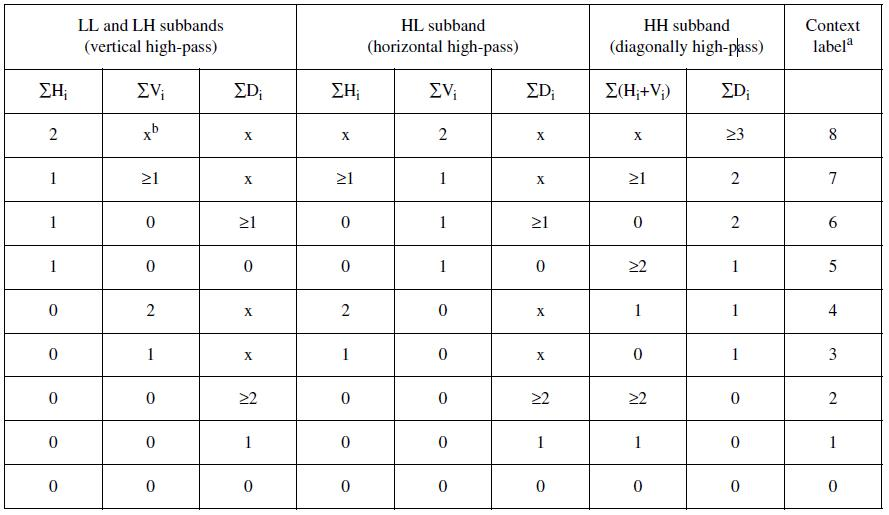
\includegraphics [width=6in]{zerocoding.jpg} 
\caption{零编码(zero coding)上下文(context)编码方式} 
\label{fig:zero coding} 
\end{figure}

\subsubsection{符号编码(Sign Coding)}
该编码根据待编码的数据比特上、下、左、右的4个相邻数据重要性情况以及待编码数据的符号位编码,返回符号编码(XORbit)和Context。具体编码规则如表{~\ref{tab:sign coding}}所示。其中“1”表示在垂直或者水平方向的相邻两个数据都为重要并且符号都为正;或者只有一个是重要的情况。“0”表示两个方向的相邻数据中两个数据都不重要或者都为重要但是具有不同的符号。-1表示的情况和1的情况相反。\textit{代码见函数SignCoding。}

\begin{table}[H]
\begin{center}
\begin{tabular}{|c|c|c|c|}
\hline
\textbf{Horizontal contribution} & \textbf{Vertical contribution} & \textbf{Context label} & \textbf{XORbit}\\
\hline
1 & 1 & 13 & 0\\
\hline
1 & 0 & 12 & 0\\
\hline
1 & -1 & 11 & 0\\
\hline
0 & 1 & 10 & 0\\
\hline
0 & 0 & 9 & 0\\
\hline
0 & -1 & 10 & 1\\
\hline
-1 & 1 & 11 & 1\\
\hline
-1 & 0 & 12 & 1\\
\hline
-1 & -1 & 13 & 1\\
\hline
\end{tabular}
\end{center}
\caption{符号编码(XORbit)和上下文(context)编码方式}
\label{tab:sign coding}
\end{table}

\subsubsection{幅度精炼编码(Magnitude Refinement Coding)}
根据该数据位是否被第一次精炼,以及$\sum H_i +  \sum V_i + \sum D_i$的值进行编码,返回D和Context。D为X的值,Context的编码规则如表{~\ref{tab:magnitude coding}}所示。\textit{代码见函数MagnitudeRefinementCoding。}

\begin{table}[H]
\begin{center}
\begin{tabular}{|c|c|c|}
\hline
\textbf{是否第一次幅度精炼编码}&\textbf{$\sum H_i +  \sum V_i + \sum D_i$}&\textbf{Context}\\
\hline
否&x&16\\
\hline
是&$\geq 1$ &15\\
\hline
是& 0 &14\\
\hline
\end{tabular}
\end{center}
\caption{幅度精炼编码(Magnitude Refinement Coding)上下文(context)编码方式}
\label{tab:magnitude coding}
\end{table}

\subsubsection{游程编码(Run Length Coding)}
仅当一个编码列(4个比特数据)的目前状态都为不重要,且相邻元素也都为不重要时,开始进行游程编码处理。这时,如果一列中的4个数据也为不重要数据,则统一编码为一个上下文编码CX=17和编码数据D=0。如果4个数据中至少有一个变为重要,则首先将其表示一个上下文CX=17和编码数据D=1。然后,编码4个数据中的第一个重要数据的位置信息(00~11)作为D,并编码上下文为CX=18。此后,编码第一个重要数据的符号位,之后数据的编码按照零编码算法进行。具体编码规则如表{~\ref{tab:runlength coding}}所示。\textit{代码见函数RunLengthCoding。}

\begin{table}[H]
\begin{center}
\begin{tabular}{|c|c|c|}
\hline
\textbf{4个比特数据}&\textbf{D}&\textbf{Context}\\
\hline
(0,0,0,0)&[0]&[17]\\
\hline
(1,x,x,x)&[1,0,0] + 符号编码+零编码 &[17,18,18]+ 符号编码+零编码\\
\hline
(0,1,x,x)&[1,0,1] + 符号编码+零编码 &[17,18,18]+ 符号编码+零编码\\
\hline
(0,0,1,x)&[1,1,0] + 符号编码+零编码 &[17,18,18]+ 符号编码+零编码\\
\hline
(0,0,0,1)&[1,1,1] + 符号编码&[17,18,18]+ 符号编码\\
\hline
\end{tabular}
\end{center}
\caption{游程编码(Run Length Coding)D和上下文(context)编码方式}
\label{tab:runlength coding}
\end{table}

\subsection{分流通道}
\subsubsection{重要性传播编码通道}
在此通道中,编码位平面中的目前状态为“无效态”,但有很大概率成为“有效态”的比特数
据。只要四周的8个比特数据有一个是重要的,就将被进行零编码(Zero Coding)。在此基础上,如果该位的比特数为1,再进行符号编码。流程图如图{~\ref{fig:twopasses}}所示。\textit{代码见函数SignifiancePropagationPass。}

\begin{figure}[H]
\centering  
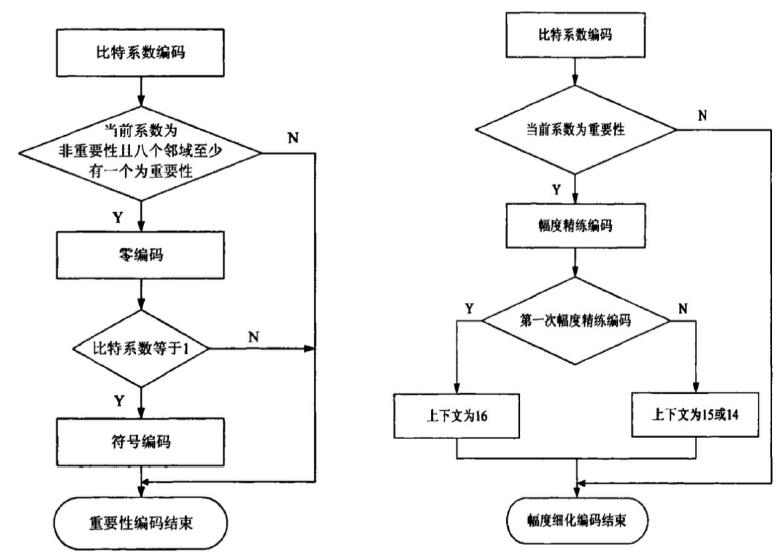
\includegraphics [width=6in]{twopasses.jpg} 
\caption{重要性传播编码通道(左)及幅度精炼编码通道(右)编码流程图} 
\label{fig:twopasses} 
\end{figure}

\subsubsection{幅度精炼编码通道}
在此通道中,编码那些在先前位平面己经被判定为有效态的数据,用“幅度精炼编码”编码。流程图如图{~\ref{fig:twopasses}}所示。\textit{代码见函数MagnitudeRefinementPass。}

\subsubsection{清除编码通道}
在此通道中,编码位平面中所有还未编码的数据。当一列4个比特都在此通道中被编码,且这4个比特都没有重要的相邻数据,则对4个比特采用游程编码(RLC),否则分别对每个比特采用零编码(Zero Coding),如数据为1,再进行符号编码(Sign Coding)。流程图如图{~\ref{fig:cleanpass}}所示。\textit{代码见函数CLeanUpPass。}

\begin{figure}[H]
\centering  
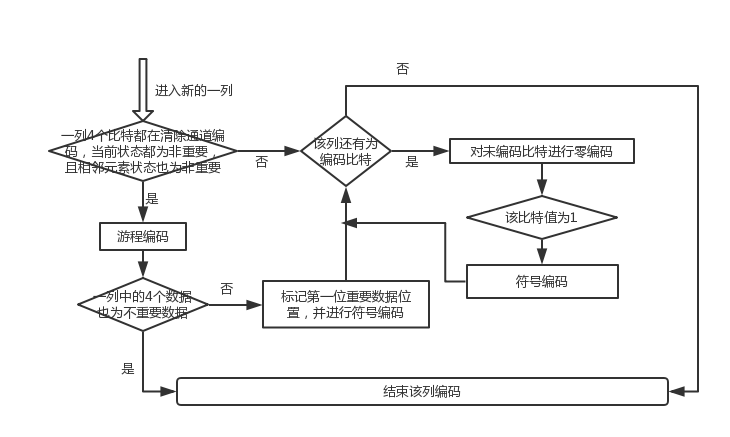
\includegraphics [width=6in]{cleanpass.jpg} 
\caption{清除编码通道编码流程图} 
\label{fig:cleanpass} 
\end{figure}

\subsection{编码流程}
\subsubsection{区段分块}
将上一步量化后的频块进一步切成32×32的区段,作为内嵌区段编码的对象,各区段之间独立运算。如频块不能被32整除,则用0补足,但是补零的同时会增加编码的冗余。

\subsubsection{位元层及符号矩阵}
对把编码区段内的数据取绝对值,依照位元深度,从高位元(MSB)到低位元(LSB)分成8个位元层。此外,由数据的正负组成符号矩阵,其中0表示正数,1表示负数。

\subsubsection{初始化上下文、重要性等矩阵}
在对整个区段编码的过程中,需要用到的矩阵及其含义如表{~\ref{tab:matrixForCoding}}所示。
\begin{table}[H]
\begin{center}
\begin{tabular}{|c|c|c|}
\hline
\textbf{矩阵(向量)名称}&\textbf{大小}&\textbf{含义}\\
\hline
重要性矩阵(S1)&32*32&表明当前状态是否为重要(用于零编码及游程编码)\\
\hline
精炼标记矩阵(S2)& 32*32 & 表明该元素是否被精炼(用于精炼编码)\\
\hline
编码标记矩阵(S3)& 32*32 & 表明该元素是否被编码(用于精炼通道及清除编码通道)\\
\hline
符号矩阵(signs)&32*32&表明该元素的符号(用于符号编码)\\
\hline
位元层(bitplanes)&X*32*32 &小波变化量化后的2进制位元表示\\
\hline
D & N*1 &编码输出矩阵\\
\hline
上下文(CX)& N*1& 编码输出上下文矩阵\\
\hline
\end{tabular}
\end{center}
\caption{编码中使用的矩阵说明}
\label{tab:matrixForCoding}
\end{table}

\subsubsection{逐位元层编码}
由高位至低位,对各位元层编码。对于各位元层,依次按照重要性传播编码通道,幅度精炼编码通道,以及清除编码通道的顺序编码。在编码各通道时,按照如图{~\ref{fig:codeorder}}所示的方式扫描。扫描过程从位平面左上角的数据开始,以4个数据为一组,连续扫描第一列的第一组4个数据后,然后转向扫描第二列的第一组4个数据,如此一直扫描到最后一列的第一组4个数据。然后,转向扫描第一列的第二组4个数据,一直到最后一列的第二组4 个数据。按照这样的顺序依次扫描整个位平面。扫描过程中矩阵的更新情况如表{~\ref{tab:matrixUpdate}}所示。\textit{代码见函数codeBlockfun。}
\begin{figure}[h]
\centering  
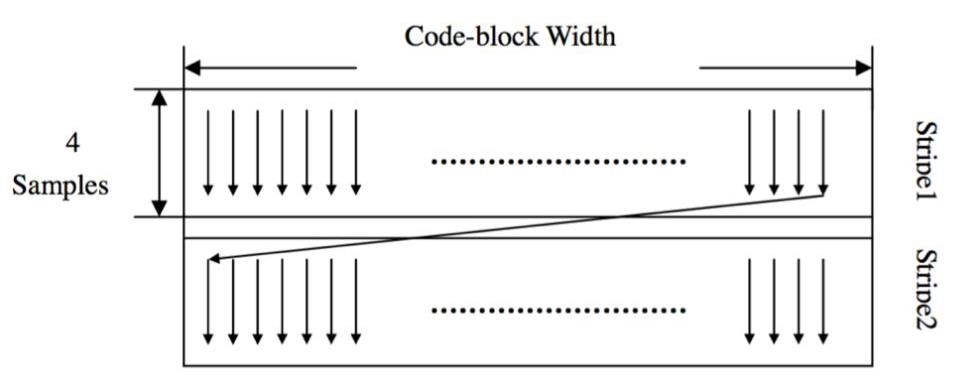
\includegraphics [width=4in]{codeorder.jpg} 
\caption{位平面扫描顺序示意图} 
\label{fig:codeorder} 
\end{figure}

\begin{table}[H]
\begin{center}
\begin{tabular}{|c|c|}
\hline
\textbf{矩阵(向量)名称}&\textbf{更新时间}\\
\hline
重要性矩阵(S1)&重要性传播编码通道及清除编码通道中更新\\
\hline
精炼标记矩阵(S2)& 精炼通道中更新\\
\hline
编码标记矩阵(S3)& 重要性传播编码通道及精炼通道中更新,结束一层位平面编码清零\\
\hline
D & 各通道都更新\\
\hline
上下文(CX)& 各通道都更新\\
\hline
\end{tabular}
\end{center}
\caption{扫描过程中矩阵的更新情况说明}
\label{tab:matrixUpdate}
\end{table}
%\section{MQ算术编解码器}
\subsection{编码器结构}
JPEG2000 所用的MQ 编码器结构如图{~\ref{fig:mqStructure}}所示。输入由待编码位D和上下文矢量CX构成,输出为压缩之后生成的码流。\\
\indent MQ编码器是一种自适应二进制算术编码器。其中,自适应算术编码是指编码系统根据已经传输和编码的信息串,调整用来划分区间的当前符号概率估计。对于同一待编码位D,其上下文CX不同,则对应的符号概率并不一定相同。因此,必须读取CX当前状态的符号概率来确定消息的符号概率,同时决定是否要转移到下一状态。符号概率的状态转移表由标准提供,共47种状态。
\begin{figure}[h]
\centering  
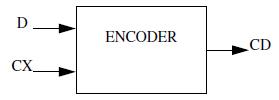
\includegraphics [width=3in]{mqStructure.jpg} 
\caption{MQ 编码器结构图} 
\label{fig:mqStructure} 
\end{figure}

\subsection{递归区间划分}
算术编码器按符号概率将符号分为大概率符号MPS和小概率符号LPS。如图{~\ref{fig:mpsLps}}所示,LPS区间在MPS区间之前。图{~\ref{fig:mpsLps}}中,A表示概率间隔长度,C表示概率间隔下限,则[C,C+A]即为编码区间。如果LPS 当前的概率估计值是Qe,编码当前符号后子区间的变化如下:\\
\indent\indent\indent如果输入符号是MPS,$ A = A * (1 - Q_e), C = C + A * Q_e$\\
\indent\indent\indent如果输入符号是LPS,$ A = A * Q_e, C 不变$\\
\indent 由于乘法运算比较费时,为简化计算,可将区间A 保持在十进制[0.75,1.5]的范围内,此时A和C可近似为:\\
\indent\indent\indent如果输入符号是MPS,$ A = A - Q_e, C = C + Q_e$\\
\indent\indent\indent如果输入符号是LPS,$ A = Q_e, C 不变$ \\
\indent 为了将A 保持在[0.75,1.5]的范围内,当整数值降到小于0.75 时,需通过重归一化把它加倍。重归一化发生时,调用概率估计模型,为当前正被编码的上下文确定一个新的概率估计。若将A 限制在十进制范围0.75~1.5 之间,概率区间的划分可以使用简单的算术近似方法。
\begin{figure}[h]
\centering  
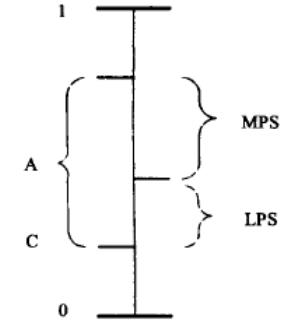
\includegraphics [width=2in]{mpsLps.jpg} 
\caption{MQ编码器编码区间示意图} 
\label{fig:mpsLps} 
\end{figure}

\subsection{编码流程}
首先对编码器进行初始化INTENC,然后读入上下文CX和待编字节D开始编码。编码时判断D是大概率符号还是小概率符号。如为大概率符号,进行CODEMPS编码;如为小概率符号,进行CODELPS编码。CODEMPS和CODELPS的编码流程如图{~\ref{fig:codemps}}和图{~\ref{fig:codelps}}所示。\textit{代码见函数entropy\_coding。}
\begin{figure}[h]
\centering  
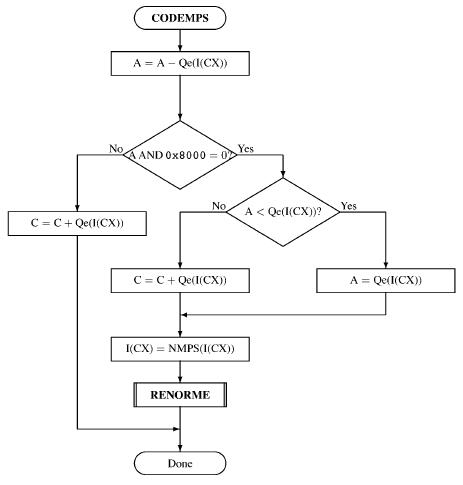
\includegraphics [width=4in]{codemps.jpg} 
\caption{CODEMPS流程图} 
\label{fig:codemps} 
\end{figure}

\begin{figure}[h]
\centering  
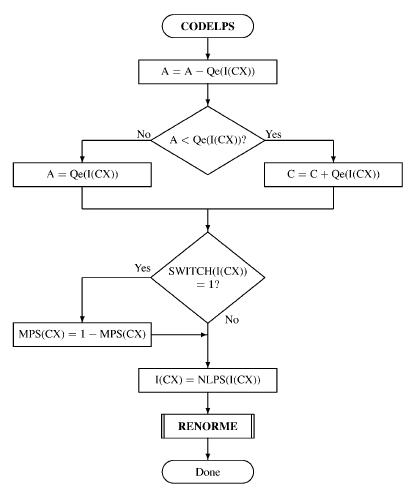
\includegraphics [width=4in]{codelps.jpg} 
\caption{CODELPS流程图} 
\label{fig:codelps} 
\end{figure}

\subsection{解码流程}
解码器根据CX和CD,一次解码一个二进制数据(如图{~\ref{fig:mqDeStructure}}所示)。同编码时一样,在解码工程中,同步调整用来划分区间的当前符号概率估计。\textit{代码见函数entropy\_decoding。}
\begin{figure}[h]
\centering  
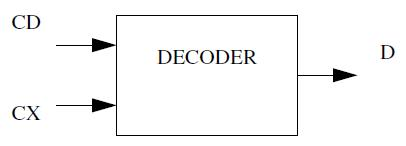
\includegraphics [width=2in]{mqDeStructure.jpg} 
\caption{MQ 解码器结构图} 
\label{fig:mqDeStructure} 
\end{figure}

\section{结果}
压缩前后大小比较、图片比较

\begin{thebibliography}{1}
\bibitem{github} jpeg2000. Jordan Van Duyne. https://github.com/jovanduy/jpeg2000.
\bibitem{book1} Taubman D , Marcellin M . JPEG2000图像压缩基础、标准和实践[M]. 电子工业出版社, 2004.
\bibitem{csdn1} CSDN:压缩算法——JPEG2000 编解码原理. 佚名. https://blog.csdn.net/ytang\_/article/details/76571635.
\bibitem{baidu} 百度文库:Daubechies 97和Le Gall 53小波分解与合成. 佚名. https://wenku.baidu.com/view/84fc5c7caaea998fcc220e7b.
\bibitem{zhihu1} 知乎:能不能通俗的讲解下傅立叶分析和小波分析之间的关系?. 佚名. https://www.zhihu.com/question/22864189/answer/40772083.
\bibitem{pywavelets} pywavelets官方文档. 佚名. https://pywavelets.readthedocs.io/en/latest/index.html.
\bibitem[7]{quantizer} P. E. Fleischer.  Sufficient  conditions for achieving minimum  distortion in a quantizer. IEEE Int. Conv. Rec., 1:104-111, 1964. 
\bibitem[8]{optimalQuantizer}Farvardin N , Modestino J W . Optimum quantizer performance for a class of non-Gaussian memoryless sources[J]. IEEE Transactions on Information Theory, 1984, 30(3):485-497.
\end{thebibliography}


\end{document}